\documentclass[12pt]{report}
\usepackage[italian]{babel}
\usepackage[most]{tcolorbox}
\usepackage{amsmath}
\usepackage{amsthm}
\usepackage{mathtools}
\usepackage{tabularx}
\usepackage{amssymb}
\usepackage{enumitem}
\usepackage{amsfonts}
\usepackage{centernot}
\usepackage{relsize}
\usepackage{mathrsfs}
\usepackage{bm}
\usepackage{xfrac}
\usepackage{xcolor}
\usepackage{lipsum}
\usepackage{bbm}
\usepackage{tikz}
\usepackage{tikz-3dplot}
\usepackage{cancel}
\usepackage{enumitem}
\usepackage{mathtools}
\usepackage{multicol}
\usepackage{float}
\usepackage{hyperref}
\usepackage{makecell}
\usepackage{listings}
\usepackage{xcolor}
\usepackage{pgfplots}
\usepackage{calligra}
\usepackage[toc,page]{appendix}
\usepackage{tikz}
\usepackage{yhmath}
\usepackage[export]{adjustbox}
\usetikzlibrary{angles, quotes, patterns}
\usepackage{circledsteps}
\date{}
\author{Alessandro Carella}
\title{Fondamenti di fisica}
%\setcounter{chapter}{0}
\setlist[enumerate]{label*=\arabic*.}
\setlength{\parindent}{0pt}
\definecolor{brickred}{RGB}{182, 50, 28}
\definecolor{darkred}{RGB}{139,0,0}
\hypersetup{
	colorlinks=true,
	linkcolor=darkred,
	filecolor=darkred,
	urlcolor=darkred
}

\newcounter{theorem}
\newcounter{lemma}
\newcounter{corollary}
\newcounter{definition}
\newcounter{exercise}

\labelformat{theorem}{teorema #1}
\labelformat{lemma}{lemma #1}
\labelformat{corollary}{corollario #1}
\labelformat{definition}{definizione #1}
\labelformat{note}{nota #1}
\labelformat{example}{esempio #1}
\labelformat{exercise}{esercizio #1}

\newtcbtheorem[number within=chapter,use counter=theorem]{theorem}%
{Teorema}{arc=1mm,outer arc=1mm,colframe=cyan!55!black,fonttitle=\scshape,lefttitle=1mm,separator sign dash,description font=\bfseries,description delimiters={\flqq}{\frqq}}{th}

\newtcbtheorem[number within=theorem,use counter=corollary]{corollary}%
{Corollario}{arc=1mm,outer arc=1mm,colframe=cyan!55!black,fonttitle=\scshape,lefttitle=1mm,separator sign dash,description font=\bfseries,description delimiters={\flqq}{\frqq}}{cor}

\newtcbtheorem[number within=chapter,use counter=lemma]{lemma}%
{Lemma}{arc=1mm,outer arc=1mm,colframe=cyan!55!black,fonttitle=\scshape,lefttitle=1mm,separator sign dash,description font=\bfseries,description delimiters={\flqq}{\frqq}}{lem}

\newtcbtheorem[number within=chapter,use counter=definition]{definition}%
{Definizione}{arc=1mm,outer arc=1mm,colframe=green!55!black,fonttitle=\scshape,separator sign dash,description font=\bfseries,description delimiters={\flqq}{\frqq}}{def}

\newtcbtheorem[no counter]
{note}{Nota}{blanker,breakable,left=5mm,before skip=10pt,after skip=10pt,borderline west={2.5mm}{0pt}{red!55},coltitle=black,fonttitle=\bfseries}{note}

\newtcbtheorem[no counter]
{example}{Esempio}{blanker,breakable,left=5mm,before skip=10pt,after skip=10pt,borderline west={2.5mm}{0pt}{yellow!55},coltitle=black,fonttitle=\bfseries}{exa}

\newtcbtheorem[number within=section,use counter=exercise]
{exercise}{Esercizio}{blanker,breakable,left=5mm,before skip=10pt,after skip=10pt,borderline west={2.5mm}{0pt}{yellow!55},coltitle=black,fonttitle=\bfseries}{exe}

\newtcbtheorem[no counter]
{assignment}{Traccia}{blanker,breakable,left=5mm,before skip=10pt,after skip=10pt,borderline west={2.5mm}{0pt}{brickred!65},coltitle=black,fonttitle=\bfseries}{asg}
\tcolorboxenvironment{proof}{blanker,breakable,left=5mm,before skip=10pt,after skip=10pt,borderline west={2.5mm}{0pt}{cyan!55!black}}
\newcommand{\namerefl}[1]{%
	\bgroup
	\let\nmu\MakeLowercase
	\nameref{#1}\egroup}

\newcommand{\nmu}{}

\begin{document}
	{
		\let\cleardoublepage\clearpage
		\maketitle
		\tableofcontents
	}
	\chapter{Ripasso formule matematiche}
	\section{Geometria}
	\subsection{Aree e volumi}
	\paragraph{Quadrato} \quad \\
	Dato un quadrato di lato L, la sua area e' pari a L$^2$. 
	\paragraph{Rettangolo} \quad \\
	Dato un rettangolo di base $a$ e altezza $b$ la sua area e' pari a $a \cdot b$. 
	\paragraph{Cubo} \quad \\
	Dato un cubo di lato L, il suo volume e' pari a L$^3$. 
	\paragraph{Parallelepipedo} \quad \\
	Dato un parallelepipedo di base $a$, altezza $b$ e profondita' $c$, il suo volume e' pari a $a \cdot b \cdot c$ 
	\paragraph{Triangolo} \quad \\
	Dato un triangolo di base $b$ e altezza $h$ la sua area e' pari a: $\dfrac{b \cdot h}{2}$ 
	\paragraph{Triangolo rettangolo} \quad \\
	Dato un triangolo rettangolo di cateti $c_1$ e $c_2$ la sua area e' pari a: $\dfrac{c_1 \cdot c_2}{2}$ 
	\paragraph{Trapezio} \quad \\
	Dato un trapezio di altezza $h$, base maggiore $b_1$ e base minore $b_2$ la sua area e' pari a: $\dfrac{(b_1 + b_2) \cdot h}{2}$ 
	\paragraph{Circonferenza} \quad \\
	Data una circonferenza di raggio $r$:
	\begin{itemize}
		\item Il diametro e' pari a $2r$ 
		\item Il perimetro e' pari a: $L = 2\pi r$
		\item L'area e' pari a: $A = \pi r^2$
	\end{itemize}
	\paragraph{Sfera} \quad \\
	Data una sfera di raggio $r$:
	\begin{itemize}
		\item La superficie della sfera e' pari a: $4\pi r^2$
		\item Il volume della sfera e' pari a: $\dfrac{4}{3}\pi r^3$
	\end{itemize}
	\paragraph{Cilindro} \quad \\
	Dato un cilindro di raggio $r$ e altezza $h$:
	\begin{itemize}
		\item L'area del cilindro e' pari a: $S_{tot} = 2S_{base} + S_{laterale} = 2\pi r^2 + 2\pi rh$
		\item Il volume del cilindro e' pari a: $V = S_{base} \cdot h = \pi r^2 h$
	\end{itemize}
	\section{Parabola}
	Una \textbf{parabola} e' l'insieme dei punti del piano equidistanti da una retta \textbf{L} (detta \textbf{direttrice}) e da un punto \textbf{F} (detto \textbf{fuoco}) non contenuto in L. 
	\begin{figure}[H]
		\centering
		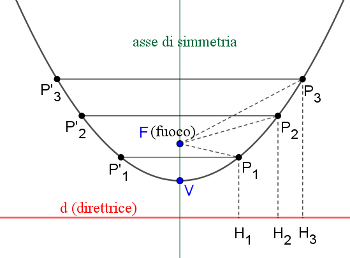
\includegraphics[width=0.5\textwidth]{parabola}
	\end{figure}
	Una parabola con asse di simmetria parallelo all'asse $y$ e' rappresentata dall'equazione:
	\[
	y = ax^2 + bx + c
	\]
	I punti importanti di una parabola sono:
	\begin{itemize}
		\item \textbf{Vertice}: $V = \Bigl(-\dfrac{b}{2a}, \dfrac{4ac - b^2}{4a}\Bigr)$
		\item \textbf{Fuoco}: $F = \Bigl(-\dfrac{b}{2a}, \dfrac{1-b^2+4ac}{4a}\Bigr)$
		\item \textbf{Asse di simmetria}: $x = -\dfrac{b}{2a}$
	\end{itemize}
	\section{Trigonometria}
	La proporzione per convertire angoli in gradi in angoli in radianti e viceversa e' la seguente:
	\[
	360^\circ\ : 2\pi\ = \alpha^\circ\ : \alpha_{rad}
	\]4
	\subsection{Funzioni trigonometriche}4
	Sia dato un triangolo rettangolo ABC, ove $c^2 = a^2 + b^2$
	\begin{figure}[H]
		\centering
		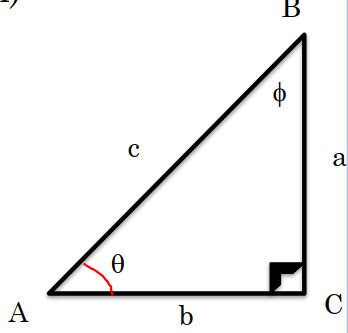
\includegraphics[width=0.5\textwidth]{triangolo_rettangolo}
	\end{figure}
	Dalla definizione della funzione seno abbiamo che:
	\[
	\sin \theta = \frac{\text{lato opposto a } \theta}{\text{ipotenusa}} = \frac{a}{c} = \frac{a}{\sqrt{a^2 + b^2}}
	\]
	Dalla definizione della funzione coseno abbiamo che:
	\[
	\cos \theta = \frac{\text{lato adiacente a } \theta}{\text{ipotenusa}} = \frac{b}{c} = \frac{b}{\sqrt{a^2 + b^2}}
	\]
	Dalla definizione della funzione tangente abbiamo che:
	\[
	\tan \theta = \frac{\text{lato opposto a } \theta}{\text{lato adiacente a } \theta} = \frac{a}{b}
	\]
	\[
	\tan \theta = \frac{\text{lato opposto a } \theta}{\text{ipotenusa}} \cdot \frac{\text{ipotenusa}}{\text{lato adiacente a } \theta} = \frac{a}{c} \cdot \frac{c}{b} = \frac{\sin \theta}{\cos \theta}
	\]
	Dalle definizioni segue che:
	\begin{itemize}
		\item $a = c \sin \theta$
		\item $b = c \cos \theta$
		\item $a_2 + b^2 = c^2\sin^2\theta+ c^2\cos^2\theta=  c^2(\sin^2\theta+\cos^2\theta) = c^2$
	\end{itemize}
	La relazione fondamentale della trigonometria e':
	\[
	\sin^2 \theta+\cos^2\theta = 1
	\]
	Dato che:
	\[
	\sin \theta = \cos(90^\circ - \theta) \quad \cos \theta = \sin(90^\circ - \theta)	
	\]
	e ricordando che: $\phi = 90^\circ - \theta$, allora:
	\begin{itemize}
		\item $a = c\cos\phi$
		\item $b = c\sin\phi$
	\end{itemize}
	\section{Prodotti di vettori}
	Siano \textbf{i}, \textbf{j}, \textbf{k} i versori dei tre assi $x, y, z$. Allora:
	\[
	\textbf{i} \cdot \textbf{i} = \textbf{j} \cdot \textbf{j} = \textbf{k} \cdot \textbf{k} = 1
	\]
	\[
	\textbf{i} \cdot \textbf{j} = \textbf{j} \cdot \textbf{k} = \textbf{k} \cdot \textbf{i} = 0
	\]
	\[
	\textbf{i} \times \textbf{i} = \textbf{j} \times \textbf{j} = \textbf{k} \times \textbf{k} = 0
	\]
	\[
	\textbf{i} \times \textbf{j}  = -\textbf{j} \times \textbf{i} = \textbf{k}
	\]
	\[\textbf{j} \times \textbf{k} = -\textbf{k} \times \textbf{j} = \textbf{i} 
	\]
	\[
	\textbf{k} \times \textbf{i} = -\textbf{i} \times \textbf{k} = \textbf{j}
	\]
	\chapter{Grandezze fisiche}
	Lo scopo della fisica e' fornire una \textbf{comprensione quantitativa} di un gran numero di fenomeni naturali che hanno luogo nel nostro universo. E' una scienza basata su osservazioni sperimentali e analisi matematiche. \\
	La fisica ricerca e formula leggi per la descrizione dei fenomeni naturali esprimendole in linguaggio matematico; il confronto tra teoria ed esperienza e' alla base di validita' di tali leggi che devono essere dotate di potere predittivo. \\
	La scienza e l'ingegneria si basano su misure e confronti tra misure. Per questo abbiamo bisogno di regoleche stabiliscano come eseguire e confrontare le misure e di esperimenti per stabilire le unita' per le misure e i confronti tra misure. Uno degli scopi della fisica e' di ideare e realizzare tali esperimenti. \\
	Scopriamo la fisica imparando a misurare le grandezze coinvolte nella fisica. Fra queste troviamo:
	\begin{itemize}
		\item la lunghezza;
		\item il tempo;
		\item la massa;
		\item la temperatura;
		\item la pressione;
		\item la corrente elettrica.
	\end{itemize}
	Misuriamo ogni grandezza fisica nelle sue unita' di misura, tramite il confronto con un \textbf{riferimento standard}. \\
	L'\textbf{unita' di misura} e' una denominazione specifica che attribuiamo alle misure di una data grandezza, ad esempio il metro e' l'unita' di misure della lunghezza. Il riferimento standard per la lunghezza e' la distanza percorsa della luce nel vuoto in una data frazione di secondo. Una volta stabilito il riferimento standard dobbiamo mettere a punto delle procedure tramite le quali qualsiasi lunghezza possa essere espressa in termini del riferimento standard. \\
	\section{Grandezze fondamentali}
	In \textbf{meccanica} le tre quantita' fondamentali sono lunghezza, massa e tempo e tutte le altre possono essere espresse in funzione di queste tre.
	Data la vastita' delle grandezze fisiche e' difficile organizzarle ma, per fortuna, queste non sono tutte indipendenti. Ad esempio, la velocita', e' il rapporto tra una lunghezza e un intervallo di tempo. Quindi, quello che facciamo e' assegnare un piccolo numero di grandezze fisiche e assegnare solo a queste dei riferimenti standard. Poi definiamo tutte le altre grandezze in base alle \textit{grandezze fondamentali} e ai loro riferimenti standard, detti \textit{standard fondamentali}. \\
	Gli standard fondamentali devono essere sia \textit{reperibili} che \textit{invariabili}. L'esigenza di precisione nela scienza e nell'ingegneria ci spinge a puntare prima di tutto all'invariabilita'.
	\section{Sistema Internazionale delle unita' di misura}
	Nel 1971, la 14$^a$ Conferenza Generale dei pesi e delle misure seleziono' sette grandezze come grandezze fondamentali, stabilendo la base del SI, il Sistema Internazionale delle unita' di misura.
	\begin{table}[H]
		\centering
		\caption{Grandezze e unità fondamentali del SI}
		\label{tab:1.1}
		\small
		\begin{tabular}{lccl}
		\hline
		Grandezza & \begin{tabular}{c}Simbolo\\della\\grandezza\end{tabular} & \begin{tabular}{c}Unità\\di misura\\corrispondente\end{tabular} & \begin{tabular}{c}Simbolo\\della unità\\di misura\end{tabular} \\
		\hline
		Lunghezza & $l$ & metro & m \\
		Massa & $m$ & chilogrammo-massa & kg \\
		Intervallo di tempo & $t$ & secondo & s \\
		Temperatura assoluta & $T$ & grado Kelvin & K \\
		Intensità luminosa & $I$ & candela & cd \\
		Intensità di corrente & $i$ & ampère & A \\
		\hline
		\end{tabular}
	\end{table}
	Nel SI molte unita' derivate sono definite in funzione delle unita' delle grandezze fondamentali. Per esempio, l'unita del SI per la potenza, chiamata \textbf{watt}, e' definita in funzione delle unita' di massa, lunghezza e tempo. \\
	Per esprimere numeri molto grandi o molto piccoli, ricorriamo alla \textit{notazione scientifica}, che usa le potenze di 10. Ad esempio:
	\[
	3\ 560\ 000\ 000\ m = 3,56 \cdot 10^9\ m
	\]
	oppure
	\[
	0, 000\ 000\ 492\ s = 4,92 \cdot 10^{-7}\ s
	\]
	Quando abbiamo a che fare con misure molto grandi o molto piccole, usiamo i prefissi elencati nella seguente tabella:
	\begin{table}[H]
		\centering
		\caption{Prefissi per le unità del SI.}
		\label{tab:prefissi_SI}
		\begin{tabular}{cll}
			\hline
			\textbf{Fattore} & \textbf{Prefisso} & \textbf{Simbolo} \\
			\hline
			$10^{24}$ & yotta- & Y \\
			$10^{21}$ & zetta- & Z \\
			$10^{18}$ & exa- & E \\
			$10^{15}$ & peta- & P \\
			$10^{12}$ & tera- & T \\
			$10^{9}$ & giga- & G \\
			$10^{6}$ & mega- & M \\
			$10^{3}$ & kilo- & k \\
			$10^{2}$ & etto- & h \\
			$10^{1}$ & deca- & da \\
			$10^{-1}$ & deci- & d \\
			$10^{-2}$ & centi- & c \\
			$10^{-3}$ & milli- & m \\
			$10^{-6}$ & micro- & $\mu$ \\
			$10^{-9}$ & nano- & n \\
			$10^{-12}$ & pico- & p \\
			$10^{-15}$ & femto- & f \\
			$10^{-18}$ & atto- & a \\
			$10^{-21}$ & zepto- & z \\
			$10^{-24}$ & yocto- & y \\
			\hline
		\end{tabular}
	\end{table}
	Ciascun prefisso rappresenta una potenza di 10, da usare come fattore moltiplicativo. Quindi, ad esempio:
	\[
	1,27 \cdot 10^9\ watt = 1,27\ gigawatt = 1,27\ GW
	\]
	Abbiamo spesso bisogno di convertire le unita' in cui una grandezza fisica  e' espressa in altre unita'. Questo si fa con un metodo chiamato \textit{conversione a catena}, nel quale moltiplichiamo la misura originaria per un opportuno \textbf{fattore di conversione}. Per esempio, poiche' 1 min e 60 s sono intervalli di tempo identici, possiamo scrivere:
	\[
	\frac{1\ min}{60\ s} = 1 \quad \frac{60\ s}{1\ min} = 1
	\]
	Percio questi due rapporti possono essere usati come fattori di conversione, tuttavia questi rapporti non equivalgono a scrivere 1/60 = 1 oppure 60 = 1; ciasun numero e la sua unita' di misura devono essere trattati insieme. \\
	Moltiplicare una qualsiasi grandezza per 1 significa lasciarla inalterata, possiamo introdurre dei fattori di conversione ogni volta che lo riteniamo utile, ad esempio per convertire 2 minuti in secondi, abbiamo:
	\[
	2\ min = (2\ min) \cdot 1 = (2\ min) \cdot \Bigl(\frac{60\ s}{1\ min}\Bigr) = 120\ s
	\]
	\section{Lunghzza}
	Nel 1792 la Replubblica Francese stabili' un niovo sistema di pesi e di misure. Il fondamento di esso era il \textit{metro}, definite come la decimilionesima parte della distanza tra il polo nord e l'equatore. Successivamente, si defini' il metro come la distanza tra due linee sottili incise vicono alle estremita' di una barra di platino-iridio, la \textbf{barra del metro campopne}. Copie di questa barra vennero mandate ai laboratori di metrologia di tutto il mondo. \\
	Col tempo si rece necessario un riferimento standard piu' preciso della distanza tra due incisioni su una barra di metallo e nel 1960 si defini' il metro come la distanza d'onda della luce. \\
	Nel 1983, serviva ancora piu' precisione e quindi il metro venne definito come la distanza percorsa dalla luce in un specifico intervallo di tempo, piu' specificatamente, il metro e' la lunghezza che la luce percorre nel vuoto in un intervallo di tempo pari a $\dfrac{1}{299\ 792\ 458}$ secondi. \\
	Quindi la velocita' della luce e' pari a:
	\[
	c = 299\ 792\ 458\ m/s
	\]
	\begin{table}[H]
		\centering
		\caption{Alcune lunghezze approssimative.}
		\label{tab:lunghezze}
		\begin{tabular}{@{}l c@{}}
			\hline
			\textbf{Misura} & \textbf{Lunghezza in metri} \\
			\hline
			Distanza della galassie di prima formazione & $2 \cdot 10^{26}$ \\
			Distanza della galassia di Andromeda & $2 \cdot 10^{22}$ \\
			Distanza della stella più vicina (Proxima Centauri) & $4 \cdot 10^{16}$ \\
			Distanza di Plutone & $6 \cdot 10^{12}$ \\
			Raggio della Terra & $6 \cdot 10^{6}$ \\
			Altezza del monte Everest & $9 \cdot 10^{3}$ \\
			Spessore di questa pagina & $1 \cdot 10^{-4}$ \\
			Lunghezza di un virus tipico & $1 \cdot 10^{-8}$ \\
			Raggio dell'atomo di idrogeno & $5 \cdot 10^{-11}$ \\
			Raggio di un protone & $1 \cdot 10^{-15}$ \\
			\hline
		\end{tabular}
	\end{table}
	
	La Tabella~\ref{tab:lunghezze} riporta un'ampia gamma di lunghezze, da quelle relative all'Universo (le prime righe) a quelle relative a oggetti piccolissimi.
	\section{Cifre significative e ficre decimali}
	Se in un problema ci troviamo di fonte a dati i cui numeri sono di due cifre queste sono dette \textbf{cifre decimali}. Tuttavia, la calcolatrice potrebbe mostrare molte piu' cifre. Le cifre in piu' sono prive di significato. Quando la prima delle cifre da scartare e' 5 o maggiore di 5, l'ultima cifra che conserviamo viene arrotondata a un'unita' in piu'. \\
	E' bene non confondere le \textit{cifre significative} con le \textit{cifre decimali}. Per esempio le lunghezze 35,6 m, 3,56m, e 0,00356 m hanno tutte tre significative ma rispettivamente una, due e cinque cifre decimali. \\
	E' bene notare che in fisica $72.4\ cm \neq 72.40\ cm \neq 72.400\ cm$ perche' il risultato di una misura e' sempre affetto da errore che dipende dallo strumento e dal metodo utilizzati e quindi si scrive:
	\[
	L = (72.4\ \pm 0.1)\ cm
	\]
	72.4 cm significa che abbiamo misurato con \textit{precisione del millimetro} e non sappiamo quanti decimetri di millimetri sia lungo il tavolo. \\
	72.40 cm significa che abbiamo misurato con \textit{precisione del decimo di millimetro} e non sappiamo quanti centesimi di millimetri sia lungo il tavolo. \\
	\subsection{Cifre significative nelle operazioni}
	Nel caso di \textbf{addizione} e \textbf{sottrazione} bisogna mantenere la posizione dell'addendo con \textbf{minore precisione}:
	\[
	13.214 + 234.6 + 7.0350 + 6.38 = 261.2
	\]
	Nell \textbf{moltiplicazione} e \textbf{divisione} bisogna utilizzare un numero di cifre significative pari al fattore che ne ha di meno:
	\[
	0.00435 \cdot 4.6 = 0.02
	\]
	\section{Tempo}
	Il tempo ha due aspetti. Per scopi civili e per alcuni scopi scientifici, vogliamo conoscere l'ora del giorno in modo da poter ordinare gli eventi in sequenza. In tante attivita' scientifiche vogliamo sapere qual e' la durata di un evento. 
	La tabella~\ref{tab:intervalli_tempo} mostra alcuni intervalli di tempo. \\
	Qualsiasi fenomeno che si ripeta puo' essere usato come riferimento standard per il tempo. La rotazione della Terra, che determina la lunghezza del giorno, e' stata usata a questo scopo per secoli. \\
	La 13$^a$ Conferenza generale sui pesi e sulle misure adotto' nel 1967 un riferimento standard per il secondo basato sull'orologio al cesio: "un secondo e' il tempo necessario alla luce (di una specifica lunghezza d'onda) emessa da un atomo di cesio-133 per effettuare 9 192 631 770 oscillazioni".
	\begin{table}[H]
		\centering
		\caption{Alcuni intervalli di tempo approssimati.}
		\label{tab:intervalli_tempo}
		\begin{tabular}{@{}p{8cm} c@{}}
			\hline
			\textbf{Misura} & \textbf{Intervallo di tempo in secondi} \\
			\hline
			Vita media di un protone (stima) & $3 \cdot 10^{40}$ \\
			Età dell'Universo & $5 \cdot 10^{17}$ \\
			Età della piramide di Cheope & $1 \cdot 10^{11}$ \\
			Aspettativa di vita di un essere umano & $2 \cdot 10^{9}$ \\
			Durata di un giorno & $9 \cdot 10^{4}$ \\
			Intervallo di tempo tra due battiti cardiaci umani & $8 \cdot 10^{-1}$ \\
			Vita media del muone & $2 \cdot 10^{-6}$ \\
			Il più breve impulso luminoso prodotto e misurato in laboratorio* & $1 \cdot 10^{-18}$ \\
			Vita media della particella più instabile & $1 \cdot 10^{-23}$ \\
			Tempo di Planck** & $1 \cdot 10^{-43}$ \\
			\hline
		\end{tabular}
	\end{table}
	\section{Massa}
	Il riferimento standard per la massa nel SI e' un cilindor di platino-iridio al quale e' stata assegnata la massa di 1 kg. La tabella ~\ref{tab:masse} mostra alcune masse espresse in kg, distribuite su un intervallo di tempo che comprende circa 83 ordini di grandezza.
	\begin{table}[H]
		\centering
		\caption{Alcune misure approssimate della massa.}
		\label{tab:masse}
		\begin{tabular}{@{}p{4cm} c p{4cm} c@{}}
			\hline
			\textbf{Oggetto} & \textbf{Massa in kg} & \textbf{Oggetto} & \textbf{Massa in kg} \\
			\hline
			Universo conosciuto & $1 \cdot 10^{53}$ & Elefante & $5 \cdot 10^{3}$ \\
			Via Lattea & $2 \cdot 10^{41}$ & Acino d'uva & $3 \cdot 10^{-3}$ \\
			Sole & $2 \cdot 10^{30}$ & Granello di polvere & $7 \cdot 10^{-10}$ \\
			Luna & $7 \cdot 10^{22}$ & Molecola di penicillina & $5 \cdot 10^{-17}$ \\
			Asteroide Eros & $5 \cdot 10^{15}$ & Atomo di uranio & $4 \cdot 10^{-25}$ \\
			Piccola montagna & $1 \cdot 10^{12}$ & Protone & $2 \cdot 10^{-27}$ \\
			Transatlantico & $7 \cdot 10^{7}$ & Elettrone & $9 \cdot 10^{-31}$ \\
			\hline
		\end{tabular}
	\end{table}
	\subsection{Bilancia di Kibble} 
	Un modo piu' accurato e' ora in uso per misurare la massa. Nella \textit{bilancia di Kibble}, dal nome dell'inventore Bryan Kibble, una massa campione puo' essere misurata quando la trazione verso il basso, dovuta alla gravita', e' bilanciata da una forza verso l'alto, dovuta a un campo magnetico indotto da una corrente elettrica. \\
	La precisione di questa tecnica viene dal fatto che le proprieta' elettriche e magnetiche possono essere determinate in termini di grandezze quantistiche che sono state misurate in modo preciso.
	\subsection{Una seconda massa di riferimento standard}
	Le masse degli atomi possono essere confrontate tra loro con precisione molto maggiore di quanto non sia possible fare confrontandole con il kilogrammo campione. \\
	Per questo abbiamo un secondo riferimento standard per la massa. Si tratta dell'atomo di carbonio-12 al quale, per accordo internazionale, e' stata attribuita la massa di 12 \textbf{unita' di massa atomica} (u). La relazione tra le due unita' e':
	\[
	1\ u = 1, 660\ 538\ 86 \cdot 10^{-27}\ kg
	\]
	con un incertezza di $\pm 10$ sulle ultime due cifre decimali. Con uno spettometro di massa gli scienziati possono, determinare la masse di altri atomi in relazione alla massa dell'atomo di carbonio-12.
	\subsection{Densita'}
	La densita' $\rho$ e' la massa per unita' di volume:
	\[
	\rho = \frac{m}{V}
	\]
	Le densita', generalmente, sono date in kilogrammi al metro cubo oppure in grammi al centrimetro cubo.
	\section{Equazioni dimensionali}
	Una \textit{equazione dimensionale} e' un'equazione dove tutti i termini sono le dimensioni delle grandezze fisiche in gioco. Ad esempio:
	\[
	velocita'\ =\ spazio/tempo
	\]
	L'equazione dimensionale e':
	\[
	[velocita']\ =\ [metri]/[secondo]
	\]
	Ogni grandezza fisica, $A$, in meccanica, puo' essere espressa in termini delle tre grandezze fondamentali:
	\[
	\text{L (Lunghezza) - T (Tempo) - M (Massa)}
	\]
	secondo l'equazione dimensionale:
	\[
	[A]\ =\ [L^\alpha\ T^\beta\ T^\gamma]
	\]
	dove gli esponenti $\alpha, \beta, \gamma$ sono numeri interi o frazionari, positivi, negativi o nulli. \\ \quad \\
	\begin{tabular}{l@{\hspace{3cm}}l}
		[area] = [L$^2$ M$^0$ T$^0$] & [velocità] = [L$^1$ M$^0$ T$^{-1}$] \\[0.5cm]
		[densità] = [L$^{-3}$ M$^1$ T$^0$] & [forza] = [L$^1$ M$^1$ T$^{-2}$]
	\end{tabular} \\ \quad \\
	Una equazione dimensionale serve a:
	\begin{itemize}
		\item \textbf{definire le unita' di misura} delle grandezze derivate
		\item \textbf{controllare la coerenza dimensione} delle relazioni matematiche che legano piu' grandezze in una legge fisica. \\
		Infatti, membro sinistro e destro dell'equazione devono avere le stesse dimensioni fisiche. \\
		Addizioni o sottrazioni sono possibili solo tra termini omogenei, mentre, e' possibile moltiplicare o dividere grandezze con dimensioni diverse. \\
		Le funzioni trigonometriche devono avere \textbf{argomenti adimensionali} e restituiscono \textbf{valori adimensionali}.
	\end{itemize}
	\chapter{Vettori}
	Iniziamo col comprendere a cosa serve il linguaggio vettoriale. \\
	In fisica si ha a che fare con molte grandezze che hanno un valore numerico ma anche una direzione e un verso per descrivere e' necessario un linguaggio matematico specifico, il linguaggio dei vettori. In fisica si hanno bisogno dei vettori anche in modi specifici per descrivere fenomeni che coinvolgono la rotazione e le forze magnetiche. 
	\section{Vettori e scalari}
	Una particella in moto su una linea retta si puo' muovere soltanto in due versi. Possiamo definire il suo moto come positivo in uno dei due versi possibili e negativo nell'altro. Pero', per una particella che si muove in tre dimensioni, un segno + e un segno - non sono piu' sufficienti per indicare il verso del suo moto. Per questo si utilizza un \textit{vettore}. \\
	Un \textbf{vettore} ha un modulo, detto anche \textit{intensita'} o \textit{ampiezza}, una direzione e un verso, e i vettori seguono alcune regole (vettoriali) di combinazione. \\
	I vettori si possono identificare tracciando una freccia al di sopra del simbolo, per esempio, $\vec{a}$ oppure in grassetto \textbf{a}. Se vogliamo indicare solo il modulo di un vettore, useremo i simboli in corsivo $a$ oppure $|\text{\textbf{a}}|$ oppure $|\vec{a}|$. \\
	Una \textbf{grandezza vettoriale} e' una grandezza fisica che un modulo, una direzione e un verso e puo' essere rappresentata con un vettore. Alcuni esempi di grandezze vettoriali sono lo spostamento, la velocita' e l'accelerazione. \\
	Non tutte le grandezze fisiche implicano una direzione. Per esempio, la temperatura, la pressione, l'energia, la massa e il tempo non puntano in una direzione. Queste grandezze sono dette grandezze \textbf{scalari} o semplicemente \textbf{scalari} e le trattiamo con le regole dell'algebra ordinaria. Uno scalare e' specificato soltanto da un valore numerico dotato di segno. \\
	La grandezza vettoriale piu' semplice e' lo spostamento,o variazione della posizione. Un vettore che rappresenta lo spostamento e' detto \textit{vettore spostamento}, analogamente si definiscono il \textit{vettore velocita'} e il \textit{vettore accelerazione}. \\
	Se una particella cambia la sua posizione, muovendosi da A a B, diciamo che subisce uno spostamento da A a B che rappresentiamo con una freccia che punta da A a B. \\
	Il vettore spostamento non ci dice nulla sul percorso che la particella compie. I vettori spostamento rappresentano l'effetto complessivo del moto, non il moto in se'.
	\begin{figure}[H]
		\centering
		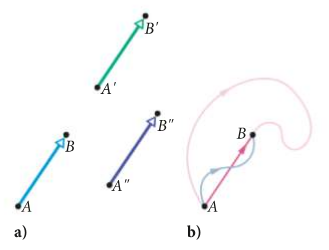
\includegraphics[width=0.5\textwidth]{vettore_spostamento}
		\caption{\textbf{a)} Le tre frecce rappresentano tutte lo stesso spostamento, avendo stesso modulo, stessa direzione e stesso verso. \textbf{b)} I tre percorsi che collegano i punti A e B corrispondono tutti allo stesso vettore spostamento}
	\end{figure}
	\section{Operazioni sui vettori}
	\subsection{Sommare due vettori geometricamente}
	\begin{figure}[H]
		\centering
		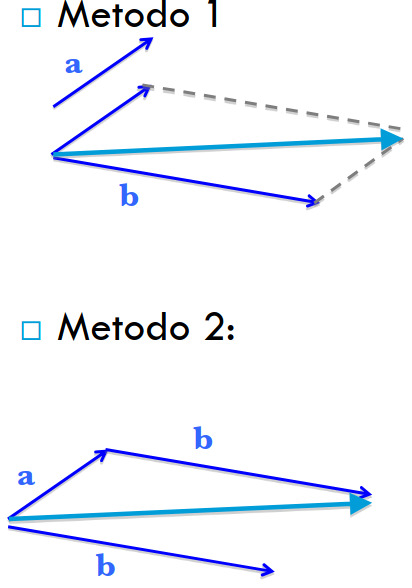
\includegraphics[width=0.5\textwidth]{somma_vettori_slide}
	\end{figure}
	Per determinare il vettore somma di \textbf{a} e \textbf{b} si possono usare due metodi:
	\begin{enumerate}
		\item Costruire un parallelogramma e il vettore somma \textbf{c = a + b} giace sulla diagonale maggiore;
		\item Unire la punta di un vettore con la coda dell'altro; unire la coda libera del primo con la punta libera del secondo.
	\end{enumerate}
	Possiamo quindi, dunque, rappresentare la relazione tra i tre vettori della figura con l'equazione vettoriale:
	\[
	\textbf{c = a + b}
	\]
	che indica che il vettore \textbf{c} e' la \textbf{somma vetoriale} dei vettori \textbf{a} e \textbf{b}. Il segno + e la parola \textit{somma} e \textit{sommare} hanno per i vettori significati diversi da quelli che hanno nell'algebra usuale, perche' coinvolgono sia il modulo sia la direzione e il verso. \\
	La somma di $n$ vettori:
	\[
	\textbf{A = A$_1$ + A$_2$ + } \dots + \textbf{A$_n$}
	\]
	e' il vettore che congiunge il primo estremo di \textbf{A}$_1$ con il secondo estremo di A$_n$, come mostrato nella figura:
	\begin{figure}[H]
		\centering
		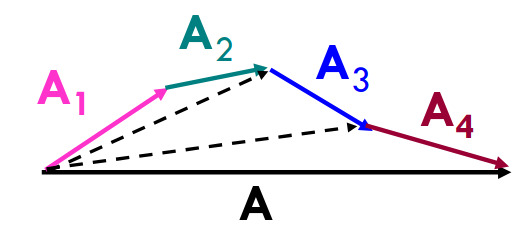
\includegraphics[width=0.5\textwidth]{somma_n_vettori}
	\end{figure}
	\paragraph{Proprieta'.} La somma vettoriale cosi' definita ha deu importanti proprieta':
	\begin{enumerate}
		\item \textbf{proprieta' commutativa}: $a + b = b + a$
		\item \textbf{proprieta' associativa}: $(a + b) + c = a + (b + c)$ \\
		\begin{figure}[H]
			\centering
			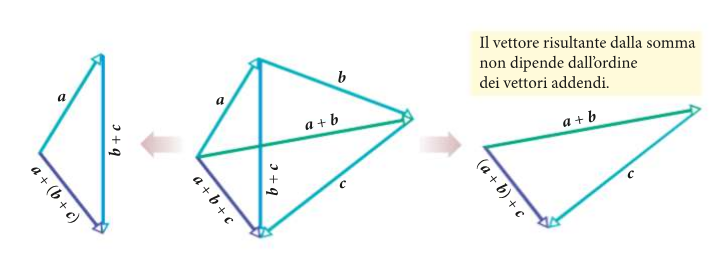
\includegraphics[width=0.75\textwidth]{proprieta_associativa}
			\caption{I tre vettori $a, b, c$ possono essere raggruppati in qualunque modo quando vengono sommati}
		\end{figure}
	\end{enumerate}
	\subsection{Sottrazione di vettori}
	Il vettore $-b$ e' un vettore che ha lo stesso modulo e la stessa direzione di $b$, ma verso opposto, come mostrato nella figura sottostante:
	\begin{figure}[H]
		\centering
		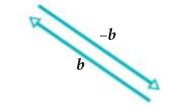
\includegraphics[width=0.3\textwidth]{differenza}
	\end{figure}
	Sommando i due vettori della figura si ottiene:
	\[
	\textbf{b + (-b)} = 0
	\]
	Quindi, sommare $-\textbf{b}$ a un vettore ha l'effetto di sottrarre \textbf{b} dallo stesso vettore. \\
	Come nell'algebra usuale, possiamo spostare un termine che contiene un vettore da un membro all'altro di un'equazione vettoriale, ma dobbiamo cambiare il segno, ad esempio:
	\[
	\textbf{d+b = a} \quad \textbf{a = d + b}
	\]
	\textbf{Possiamo sommare vettori solo dello stesso tipo}, ad esempio, possiamo sommare due spostamenti o due velocita' ma non uno spostamento e una velocita'.
	\section{Componenti di un vettore}
	Sommare i vettori graficamente puo' essere macchinoso. Una tecnica piu' semplice implica l'uso dell'algebra, ma richiede che i vettori siano posti in un sistema di assi ortogonali.
	\begin{figure}[H]
		\centering
		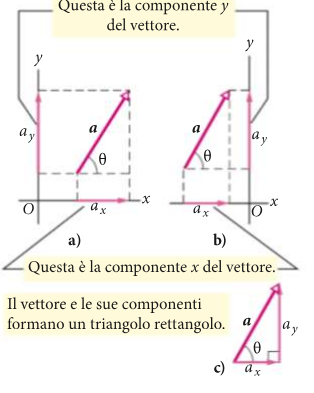
\includegraphics[width=0.4\textwidth]{piano_cartesiano}
		\caption{\textbf{a)} Le componenti $a_x$ e $a_y$ del vettore. \textbf{b)} Le componenti non cambiano se il vettore viene traslato, purche' siano mantenuti invariati il modulo e l'orientazione del vettore. \textbf{c)} Le componenti del vettore sono i cateti di un triangolo rettangolo la cui ipotenusa e' il modulo del vettore}
	\end{figure}
	Gli assi $x$ e $y$ sono tracciati nel piano della pagina. L'asse $z$ passa per l'origine ed e' perpendicolare alla pagina. \\
	La \textbf{componente} di un vettore e' la proiezione del vettore su un asse. Ad esempio, nella figura soprastante, $a_x$ e' la componente del vettore $\textbf{a}$ sull'asse delle $x$, idem per $y$. \\
	Per trovare le proiezioni di un vettore lungo un asse tracciamo dagli estremi del vettore le semirette perpendicolari agli assi. Il procedimento per trovare le componenti di un vettore prende il nome di \textbf{scomposizione del vettore}. \\
	La componente di un vettore ha la stessa direzione e lo stesso verso del vettore stesso. In generale, un vettore ha tre componenti come mostrato nella figura. 
	\subsection{Trovare le componenti} 
	Nella figura soprastante, possiamo facilmente trovare le componenti di $\mathbf{a}$ per via geometrica sul triangolo tracciato:
	\[
	a_x = \textbf{a} \cdot \cos\theta \quad a_y = \textbf{a} \cdot \sin\theta
	\]
	dove $\theta$ e' l'angolo che il vettore $\mathbf{a}$ forma con la direzione positiva dell'asse $x$ e $a$ il modulo di $\mathbf{a}$. La figura soprastante mostra che $\mathbf{a}$ e le sue componenti formano un triangolo rettangolo e mostra, inoltre, come sia possibile ricostruire un vettore a partire dalle sue componenti. \\
	Una volta che il vettore e' stato scomposto lungo gli assi di un sistema cartesiano, si possono usare le componenti stessi al posto del vettore. Per esempio, il vettore $\mathbf{a}$ della figura e' completamente determinato da $a$ e $\theta$ e puo' anche essere individuato dalle sue componenti $a_x$ e $a_y$. Se conosciamo un vettore nella \textit{notazione in componenti} ($a_x$ e $a_y$) e lo vogliamo esprimere nella \textit{notazione con modulo e angolo} ($a$ e $\theta$), per trasformarlo possiamo usare le equazioni che seguono:
	\[
	a = \sqrt{a_x^2 + a_y^2} \quad \tan \theta = \frac{a_y}{a_x}
	\]
	Nel caso piu' generale di vettori tridimensionali, per specificare un vettore ci occorrono un modulo e due angoli, per esempio $a$, $\theta$ e $\phi$ oppure tre componenti $a_x$, $a_y$ e $a_z$. \\
	Ad esempio: 
	\begin{center}
		\tdplotsetmaincoords{70}{110}
		\begin{tikzpicture}[tdplot_main_coords, scale=2]
	
		% Axes
		\draw[thick,-stealth] (0,0,0) -- (3,0,0) node[anchor=north east]{$x$};
		\draw[thick,-stealth] (0,0,0) -- (0,3,0) node[anchor=north west]{$y$};
		\draw[thick,-stealth] (0,0,0) -- (0,0,2.5) node[anchor=south]{$z$};
		
		% Vector endpoint
		\coordinate (V) at (1.5,2,1.8);
		
		% Dashed projection lines
		\draw[dashed, gray] (V) -- (1.5,2,0);
		\draw[dashed, gray] (V) -- (0,2,1.8);
		\draw[dashed, gray] (V) -- (1.5,0,1.8);
		\draw[dashed, gray] (1.5,2,0) -- (0,2,0);
		\draw[dashed, gray] (1.5,2,0) -- (1.5,0,0);
		
		% Component vectors (thick dark red/brown)
		\draw[-stealth, line width=2pt, color=brown!70!red] (0,0,0) -- (1.5,0,0) 
		node[midway, below left, black] {$\mathbf{V_x}$};
		\draw[-stealth, line width=2pt, color=brown!70!red] (0,0,0) -- (0,2,0) 
		node[midway, below right, black] {$\mathbf{V_y}$};
		\draw[-stealth, line width=2pt, color=brown!70!red] (0,0,0) -- (0,0,1.8) 
		node[midway, left, black] {$\mathbf{V_z}$};
		
		% Main vector (bright red)
		\draw[-stealth, line width=2.5pt, color=red] (0,0,0) -- (V) 
		node[midway, above left, black] {$\mathbf{V}$};
		
	\end{tikzpicture}
	\end{center}
	
	ove $\textbf{V}(V_x, V_y, V_z)$ e $V_x = x_p$, $V_y = y_p$ e $V_z = z_p$. 
	Se il primo estremo di \textbf{V} non coincide con O, come nella figura:
	\begin{figure}[H]
		\centering
		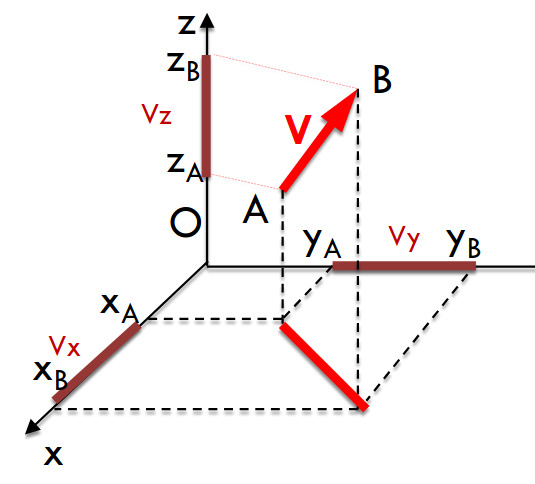
\includegraphics[width=0.5\textwidth]{estremo_neqO}
	\end{figure}
	
	allora: V = lunghezza (AB), $A(x_A, y_A, z_A)$ e $B(x_B, y_B, z_B)$ e:
	\begin{itemize}
		\item $V_x = x_B - x_A$
		\item $V_y = y_B - y_A$
		\item $V_z = z_B - z_A$
	\end{itemize}
	\section{Versori}
	Un \textbf{versore} e' un vettore che ha modulo uguale a 1 e punta in una particolare direzione e in un particolare verso. E' privo di dimensioni e di unita' di misura, il suo scopo e' uqello di indicare una direzione e un verso. I versori nel verso positivo degli assi $x, y, z$ sono indicati con i simboli \textbf{i}, \textbf{j} e \textbf{k}. \\
	I versori soni molto utili per descrivere altri vettori, ad esempio, possiamo descrivere i vettori \textbf{a} e \textbf{b} come:
	\[
	\textbf{a} = a_x\textbf{i} + a_y \textbf{j}
	\]
	e 
	\[
	\textbf{b} = b_x\textbf{i} + b_y\textbf{j}
	\]
	Le quantita' $a_x$\textbf{i} e $a_y$\textbf{j} sono le \textbf{componenti vettoriali} di \textbf{a}, da non confondere con $a_x$ e $a_y$ che sono le \textbf{componenti scalari} di \textbf{a} o semplicemente \textbf{componenti}.
	\subsection{Sommare i vettori tramite le componenti}
	Siano:
	\[
	\textbf{A}(\text{A}_x, \text{A}_y, \text{A}_z) \quad \textbf{B}(\text{B}_x, \text{B}_y, \text{B}_z)
	\]
	si definisce il vettore somma \textbf{C = A + B} di componenti $\textbf{C}(\text{C}_x, \text{C}_y, \text{C}_z)$, ove:
	\begin{itemize}
		\item C$_x$ = A$_x$ + B$_x$
		\item C$_y$ = A$_y$ + B$_y$
		\item C$_z$ = A$_z$ + B$_z$
	\end{itemize}
	\section{Moltiplicare i vettori}
	\subsection{Prodotto tra un vettore ed uno scalare}
	Sia \textbf{A} un vettore ed $m$ uno scalare. Si definisce \textbf{B} come prodotto di $m$ per \textbf{A}.
	\[
	\textbf{B} = m\textbf{A} \quad \text{vettore parallelo ad \textbf{A}}
	\]
	\[
	|\textbf{B}| = |m||\textbf{A}|
	\]
	Il verso di \textbf{B} e' concorde al verso di \textbf{A} se $m \geq 0$ mentre e' opposto al verso di \textbf{A} se $m < 0$. \\
	\subsection{Prodotto scalare tra vettori}
	\begin{figure}[H]
		\centering
		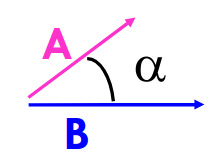
\includegraphics[width=0.5\textwidth]{prodotto_scalare}
	\end{figure}
	Il \textbf{prodotto scalare} dei vettori \textbf{a} e \textbf{b} si scrive: $\textbf{a} \cdot \textbf{b}$, si legge "a scalare b" ed e' definito dall'espressione:
	\[
	\textbf{a} \cdot \textbf{b} = ab\cos \alpha
	\]
	ove $a$ e' il modulo di \textbf{a} e $b$ il modulo di \textbf{b} e $\alpha$ l'angolo tra \textbf{a} e \textbf{b}. \\
	L'espressione puo' avere valore 0 in tre casi:
	\begin{itemize}
		\item $a$ = 0
		\item $b = 0$
		\item $\textbf{a} \perp \textbf{b}$ e quindi $\alpha = 90^\circ$ e $\cos \alpha = 0$
	\end{itemize}
	Inoltre $\textbf{a} \cdot \textbf{a} = aa \cdot \cos 0 = a^2$
	\paragraph{Proprieta' del prodotto scalare} \quad \\
	Il prodotto scalare gode della \textbf{proprieta' commutativa}:
	\[
	\textbf{a} \cdot \textbf{b} = \textbf{b} \cdot \textbf{a}
	\] 
	e della \textbf{proprieta' distributiva}:
	\[
	\textbf{a} \cdot (\textbf{b} + \textbf{c}) = \textbf{a} \cdot \textbf{b} + \textbf{a} \cdot \textbf{c}
	\]
	Inoltre, quando i due vettori sono scritti con la notazione dei versori, possiamo scrivere il loro prodotto scalare come:
	\[
	\textbf{a} \cdot \textbf{b} = (a_x\textbf{i} + a_y\textbf{j} + a_z\textbf{k}) \cdot (b_x\textbf{i}+b_y\textbf{j}+b_z\textbf{k}) = a_xb_x + a_yb_y + a_zb_z
	\]
	\subsection{Prodotto vettoriale di due vettori}
	\begin{figure}[H]
		\centering
		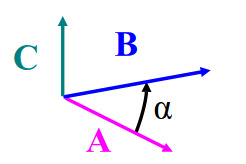
\includegraphics[width=0.5\textwidth]{prodotto_vettoriale}
	\end{figure}
	Il prodotto vettoriale di \textbf{a} e \textbf{b}, si scrive $\textbf{a} \times \textbf{b}$ e si legge "a vettore b" e' un vettore \textbf{c} il cui modulo e' dato dall'equazione:
	\[
	c = ab\sin\alpha
	\]
	La direzione di \textbf{c} e' perpendicolare al piano individuato da \textbf{a} e \textbf{b} e il verso di \textbf{c} e' definito dalla regola della vite destrorsa o della regola della mano destra. 
	\paragraph{Regola della vite}: Direzione perpendicolare al piano e verso pari allo spostamento della vite se ruotata da \textbf{a} a \textbf{b}
	\paragraph{Regola della mano destra} \quad \\
	\begin{enumerate}
		\item Supponiamo che la nostra mano destra sia il piano in cui sono disegnati i vettori;
		\item Consideriamo le prime 3 dita della mano destra: pollice, indice e medio;
		\item Orientiamo l'indice secondo la direzione di \textbf{a} e il medio secondo la direzione di \textbf{b};
		\item Orientiamo il pollice in modo che sia perpendicolare al piano  formato dalle altre 2 dita;
		\item La direzione e il verso del vettore prodtto sono quelli del pollice.
	\end{enumerate}
	\paragraph{Proprieta' del prodotto vettoriale} \quad \\
	Il prodotto vettoriale gode della \textbf{proprieta' anticommutativa}:
	\[
	\textbf{a} \times \textbf{b} = -\textbf{b} \times \textbf{a}
	\]
	e della \textbf{proprieta' distributiva}:
	\[
	\textbf{a} \times (\textbf{b} + \textbf{c}) = \textbf{a} \times \textbf{b} + \textbf{a} \times \textbf{c}
	\]
	Inoltre, se i due vettori sono descritti secondo la notazione dei versori, allora:
	
	\begin{align*}
	\textbf{a} \times \textbf{b} = (a_x\textbf{i}+ a_y\textbf{j}+ a_z\textbf{k}) \times (b_x\textbf{i} + b_y\textbf{j} + b_z\textbf{k}) &= \\ a_xb_y\textbf{k} - a_xb_z\textbf{j} - a_yb_x\textbf{k} + a_yb_z \textbf{i} + a_zb_x\textbf{i} - a_zb_y\textbf{i} &= \\ (a_yb_z - a_zb_y)\textbf{i} + (a_zb_x - a_xb_z)\textbf{j} + (a_xb_y - a_yb_x)\textbf{k}	
	\end{align*}
	\section{Derivata di un vettore}
	Dato un vettore \textbf{A}, $\dfrac{d\textbf{A}}{dt}$ e' un vettore.
	\[
	\frac{d\textbf{A}}{dt} = \lim_{\Delta t \to 0} = \frac{\textbf{A}(t + \Delta t) - \textbf{A(t)}}{\Delta t} = \lim_{\Delta t \to 0} \frac{\Delta \textbf{A}}{\Delta t}
	\]
	\[
	\frac{d(\textbf{A} + \textbf{B})}{dt} = \frac{d\textbf{A}}{dt} + \frac{d\textbf{B}}{dt}
	\]
	\[
	\frac{d(m\textbf{A})}{dt} = m\frac{d\textbf{A}}{dt} + \textbf{A}\frac{dm}{dt}
	\]
	Se $m$ e' una costante allora:
	\[
	\frac{d(m\textbf{A})}{dt} = m\frac{d\textbf{A}}{dt}
	\]
	\[
	\frac{d}{dt}(\textbf{A} \cdot \textbf{B}) = \frac{d\textbf{A}}{dt}\cdot \textbf{B} + \textbf{A} \cdot \frac{d\textbf{B}}{dt}
	\]
	\[
	\frac{d}{dt}(\textbf{A} \times \textbf{B}) = \frac{d\textbf{A}}{dt} \times \textbf{B} + \textbf{A} \times \frac{d\textbf{B}}{dt}
	\]
	In termini di componenti cartesiane, se $i, j$ e $k$ sono costanti:
	\[
	\frac{d\textbf{A}}{dt} = \frac{dA_x}{dt}\textbf{i} + \frac{dA_y}{dt}\textbf{j} + \frac{dA_z}{dt}\textbf{k}
	\]
	In generale:
	\[
	\frac{d\textbf{A}}{dt} = \frac{dA_x}{dt}\textbf{i} + \frac{dA_y}{dt}\textbf{j} + \frac{dA_z}{dt}\textbf{k} + A_x\frac{d\textbf{i}}{dt} + A_y\frac{d\textbf{j}}{dt} + A_z\frac{d\textbf{k}}{dt}
	\]
	\chapter{Cinematica unidimensionale}
	\section{Introduzione alla meccanica}
	La meccanica tratta lo studio del moto di un corpo e delle cause che lo determinano. \\
	La cinematica si suddivide in:
	\begin{itemize}
		\item \textit{cinematica}, essa si occupa di descrivere \textit{quantitativamente} il moto dei corpi, indipendentemente dalle cause del moto;
		\item \textit{dinamica}, essa e' il ramo della meccanica che si occupa dello studio delle cause del moto dei corpi, o, delle circostanze che lo determinano e lo modificano;
		\item \textit{statica}, essa e' il ramo della meccanica che si occupa dello studio delle \textit{condizioni di equilibrio}.
	\end{itemize}
	\subsection{Cinematica}
	La \textit{cinematica} e' quel ramo della meccanica che si occupa di descrivere quantitativamente il moto dei corpi, indipendentemente dalle cause del moto. \\
	Per semplicita' considereremo come corpo un punto materiale. \\
	Ad esempio, non possiamo partire dal moto di una bicicletta in quanto e' troppo complicato perche' e' un corpo esteso, non omogeneo, sono coinvolte piu' dimensioni come la rotazione, traslazione ecc. \\
	Per semplificare le cose approssimiamo i punti materiali e consideriamo gli oggetti \textit{puntiformi} che possono solo traslare e non ruotare e consideriamo moti \textit{unidimensionali} o \textit{rettilinei}, cioe' che si svolgono in un un'unica dimensione.
	\section{Moto rettilineo}
	\subsection{Posizione e spostamento}
	Localizzre un oggetto significa trovarne la posizione rispetto a un punto di riferimento, che spesso e' l'\textbf{origine} di un asse. \\
	Il primo passo, quindi, nella descrizione del moto di una particella costante consiste nello stabilire un sistema di coordinate che definiscono la sua posizione. Inoltre, e' bene anche comprendere il concetto di \textit{traiettoria}, che non e' altro che la successione delle posizioni occupate dal punto materiale durante il moto. \\
	\begin{figure}[H]
		\centering
		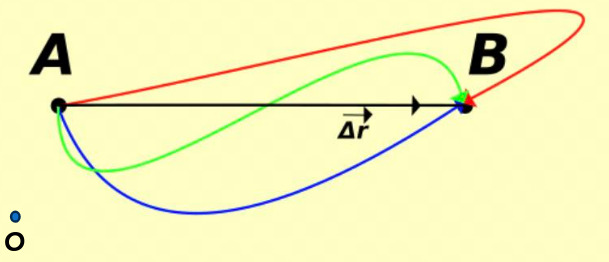
\includegraphics[width=0.5\textwidth]{vettore_posizione}
	\end{figure}
	Un cambiamento dalla posizione $x_1$ alla posizione $x_2$ e' chiamata \textbf{spostamento} $\Delta x$:
	\[
	\Delta x = x_2 - x_1
	\]
	Lo spostamento e' una \textbf{grandezza vettoriale}, quindi caratterizzata da una direzione, un verso e un modulo, ove:
	\begin{itemize}
		\item il modulo del vettore spostamento rappresenta la distanza;
		\item la direzione con il verso rappresenta se il moto avviene lungo un asse.
	\end{itemize}
	\paragraph{Vettore posizione} \quad \\
	Il punto materiale si muove lungo una retta ove $O$ e' l'origine del sistema di riferimento e $P$ e' la posizione occupata dal punto materiale all'istante di tempo $t$. Il vettore posizione all'istante di tempo $t$ e': 
	\[
	\textbf{x}(t) \text{ oppure } x(t)\textbf{i}
	\]
	e quindi e' la coordinata del punto $P$.
	\paragraph{Vettore spostamento} ]\quad \\
	Sia $Q$ la posizione occupata dal punto materiale all'istante $t + \Delta t$ e $x(t + \Delta t)$ e' la coordinata del punto  $Q$ e quindi il vettore posizione all'istante $t + \Delta t$. \\
	Lo spostamento e' il vettore differenza tra i due vettori posizione:
	\[
	\textbf{$\Delta$ x} = \textbf{x}(t + \Delta t) - \textbf{x}(t) \text{ oppure } \Delta x\textbf{i} 
	\]
	\subsection{Velocita' istantanea: vettoriale e scalare}
	All'espressione "a che velocita'" sono associate diverse grandezze, una di queste e' la \textbf{velocita' media}
	\paragraph{Velocita' media} \quad \\
	La \textit{velocita' media}, $\mathbf{v}_m$ e' il rapporto fra lo spostamento $\Delta x$ e l'intervallo di tempo $\Delta t$ nel quale avviene tale spostamento:
	\[
	\mathbf{v}_m = \frac{\mathbf{x}(t + \Delta t) - \mathbf{x}(t)}{\Delta t}  = \frac{\Delta x}{\Delta t}\mathbf{i}
	\]
	Un'unita' di misura comunemente usata per $\mathbf{v}_m$ e' il metro al secondo $m/s$. \\
	Riportiamo in un piano ($x, t$) le posizioni occupate dal punto in funzione del tempo, come in figura:
	\begin{figure}[H]
		\centering
		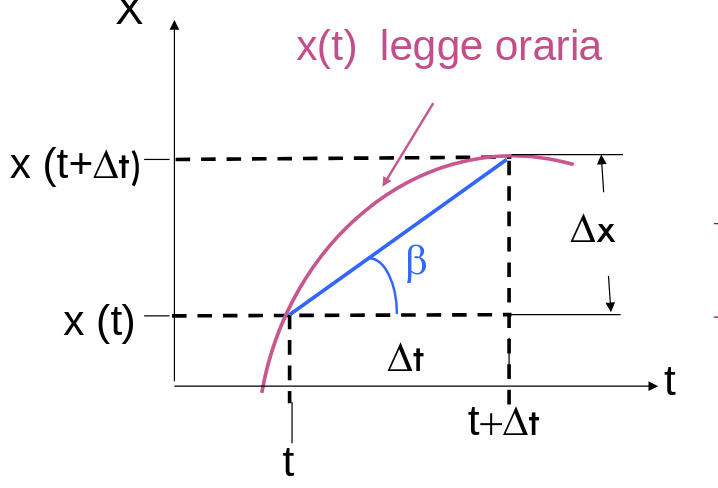
\includegraphics[width=0.5\textwidth]{diagramma_orario}
	\end{figure}
	$\mathbf{v}_m$ e' la \textbf{pendenza} della retta che unisce i punti della curva $x(t)$. Come lo spostamento anche la velocita' media e' una grandezia vettoriale, caratterizzata, quindi, da direzione, modulo e verso
	La direzione di $v_M$ e' rappresentata graficamente dalla direzione di $\tan \beta$, dove $\beta$ e' l'angolo tra l'asse orizzontale e la secante alla curva $x(t)$. 
	\paragraph{Velocita' vettoriale istantanea} \quad \\
	Di solito, l'espressione "a che velocita" si riferisce alla velocita' di una particella in un dato istante, cioe' alla sua \textbf{velocita' istantanea} o semplicemente \textbf{velocita'}. \\
	La velocita' in un qualunque istante $t$ si ottiene dalla velocita' media riducendo l'intervallo di tempo $\Delta t$ in modo di avvicinarsi sempre di piu' allo zero. Man mano che $\Delta t$ diminuisce, la velocita' media si avvicina a un valore limite che e' la velocita' in quell'istante:
	\[
	\mathbf{v}(t) = \lim_{\Delta t\to 0}\mathbf{v}_m = \lim_{\Delta t \to 0} \frac{\mathbf{x}(t + \Delta t) - \mathbf{x}(t)}{\Delta t} = \frac{\Delta x}{\Delta t}\mathbf{i} = \frac{dx(t)}{dt}\mathbf{i} 
	\]
	Quindi la velocita' vettoriale istantanea e' la derivata rispetto al tempo del vettore posizione. Inoltre, a ogni istante $t$, la velocita' $v$ e' la pendenza della retta tangente al grafico posizione-tempo della particella nel punto di ascissa $t$. Anche la velocita' istantanea e' una grandezza vettoriale, alla quale sono associate una direzione e un verso, oltre al modulo. \\
	\paragraph{Velocita' vettoriale scalare} \quad \\
	La \textbf{velocita' vettoriale scalare} o semplicemente \textbf{velocita' scalare} e' il valore assoluto della velocita' istantanea, quindi e' il \textbf{modulo} della velocita' istantanea vettoriale, senza alcun cenno alla direzione. Ad esempio, il tachimetro di un'automobile misura la velocita' scalare.
	\subsection{Accelerazione media e istantanea}
	Quando la velocita' di una particella varia, si dice che la particella e' sottoposta a un'\textbf{accelerazione}. \\
	Per il moto lungo un asse, l'\textbf{accelerazione media}, $\textbf{a}_m$ durante un intervallo di tempo $\Delta t$ e':
	\[
	\textbf{a}_m = \frac{v_2 - v_1}{t_2 - t_1} = \frac{\textbf{v}(t + \Delta t) - \textbf{v}(t)}{\Delta t} = \frac{\Delta v}{\Delta t}\textbf{i}
	\]
	in cui la particella ha velcita' $v_1$ all'istante $t_1$ e velocita' $v_2$ all'istante $t_2$. \\
	L'\textbf{accelerazione istantanea} o semplicemente \textbf{accelerazione} e' la derivata della velocita' rispetto al tempo:
	\[
	\textbf{a}(t) = \lim_{\Delta t \to 0}\textbf{a}_m = \lim_{\Delta t \to 0}\frac{\textbf{v}(t + \Delta t) - \textbf{v}(t)}{\Delta t} = \frac{dv(t)}{dt}\textbf{i}
	\]
	Quindi, l'accelerazione di una particella a un certo istante e' la rapidita' di variazione della sua velocita' a quell'istante. Graficamente, e' la pendenza della curva $v(t)$ in quel punto. \\
	Sapendo che la velocita' e' la derivata dello spostamento rispetto al tempo otteniamo:
	\[
	\textbf{a}(t) = \frac{dv(t)}{dt}\textbf{i} = \frac{d}{dt}\Bigg(\frac{dx(t)}{dt}\Bigg)\textbf{i} = \frac{d^2x(t)}{dt^2}\textbf{i}
	\]
	Ovvero, l'accelerazione di una particella in un certo istante e' la derivata seconda della sua posizione rispetto al tempo. \\
	L'unita di misura dell'accelerazione piu' comunemente usata e' il metro al secondo quadrato ($m/s^2$). \\
	L'accelerazione e' un'altra grandezza vettoriale.
	\subsection{Moto rettilineo uniforme}
	Un corpo si muove di moto rettilineo uniforme se si sposta lungo una retta con velocita' costante nel tempo.
	Quando $|\textbf{v}|$ e' costante e anche la sua direzione e' costante, vuol dire che \textbf{v} e' un vettore costante. Quando la velocita' e' costante allora $\textbf{a} = 0$. \\
	Sappiamo che:
	\[
	dx(t) = v(t)dt \quad x(t_0) = x_0
	\]
	Con quest possiamo definire la \textbf{legge oraria del moto uniforme}:
	\[
	x(t) - x_0 = \int_{x_0}^{x(t)}dx(t) = \int_{t_0}^{t}vdt = v\int_{t_0}^{t}dt \Rightarrow x(t)=x_0 + v(t-t_0)
	\]
	Se $t_0 = 0$ allora:
	\[
	x(t) = x_0 + vt
	\]
	\paragraph{Grafici del moto rettilineo uniforme} \quad \\
	\begin{figure}[H]
		\centering
		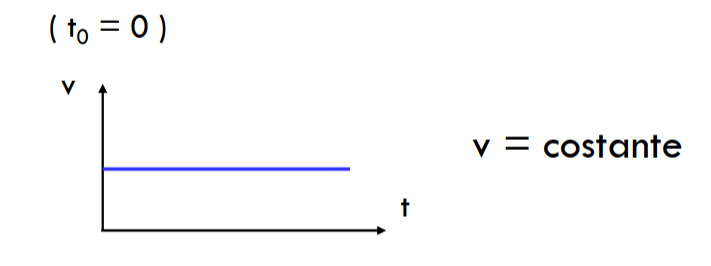
\includegraphics[width=0.7\textwidth]{mru_vCostante}
	\end{figure}
	\begin{figure}[H]
		\centering
		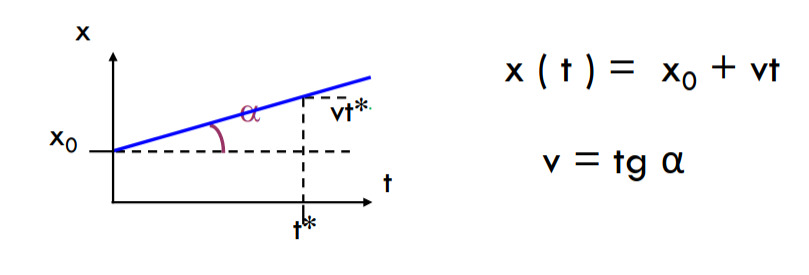
\includegraphics[width=0.7\textwidth]{mru_leggeoraria}
	\end{figure}
	\subsection{Moto rettilineo uniformemente accelerato} 
	In molti tipi di moto l'accelerazione e' costante o pressoche' costante. In questi casi si parla di \textbf{moto rettilineo uniformemente accelerato}. \\
	Quindi sappiamo che:
	\[
	\textbf{a} = \text{costante} \quad v(t_0) = v_0
	\]
	Quindi possiamo ricavarci l'equazione della velocita' come:
	\[
	v(t) - v_0 = \int_{v_0}^{v_t}dv(t)=\int_{t_0}^{t}adt
	\]
	allora:
	\[
	v(t) = v_0 + a(t - t_0)
	\]
	e se $t_0 = 0 \Rightarrow v(t) = v_0 + at$. \\
	Trovata l'equazione della velocita' possiamo trovare l'equazione dello spostamento:
	\begin{align*}
	x(t) = x_0 + \int_{t_0}^{t}dv(t) &= \\ x_0 + \int_{t_0}^{t}[v_0 + a(t - t_0)]dt &=\\ x_0 + v_0\int_{t_0}^{t}dt + a\int_{t_0}^{t}(t-t_0)dt &= \\ \Rightarrow x(t) =  x_0 + v_0(t-t_0) + \frac{1}{2}a(t-t_0)^2
	\end{align*}
	questa e' la \textbf{legge oraria del moto uniformemente accelerato}. \\
	In un moto uniformemente accelerato $v$ e' funzione della posizione $x$ oltreche del tempo e quindi, dalle equazioni precedenti possiamo ricavare altre equazioni utili. Prima di procedere, notiamo che:
	\begin{itemize}
		\item derivando $x(t)$ rispetto al tempo, otteniamo: $v(t) = \frac{dx}{dt} = v_0 + at$
		\item derivando $v(t)$ rispetto al tempo, otteniamo: $a(t) = \frac{dv}{dt} = \frac{dv}{dx}\frac{dx}{dt} = v\frac{dv}{dx}$
	\end{itemize}
	Integrando $a$ nell'intervallo $x_0$ e $x$ otteniamo:
	\[
	\int_{x_0}^{x}adx = \int_{x_0}^{x}v\frac{dv}{dx}dx = \int_{v_0}^{v}vdv=\frac{1}{2}v^2 - \frac{1}{2}v_0^2 
	\]
	allora:
	\[
	a(x - x_0) = \frac{1}{2}v^2 - \frac{1}{2}v_0^2	
	\]
	\paragraph{Grafici del moto uniformemente accelerato} \quad \\
	\begin{figure}[h]
		\centering
		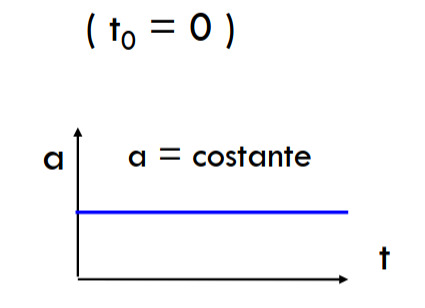
\includegraphics[width=0.4\textwidth]{mrua_aCostante}
		\hfill
		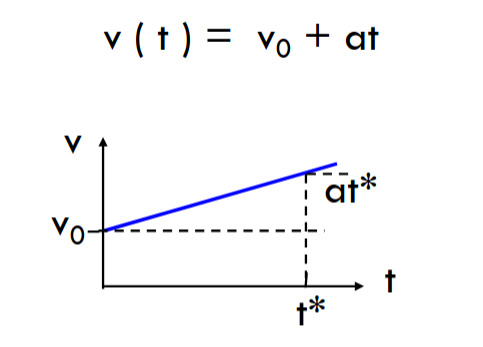
\includegraphics[width=0.4\textwidth]{mrua_velocita}
	\end{figure}
	\begin{figure}[H]
		\centering
		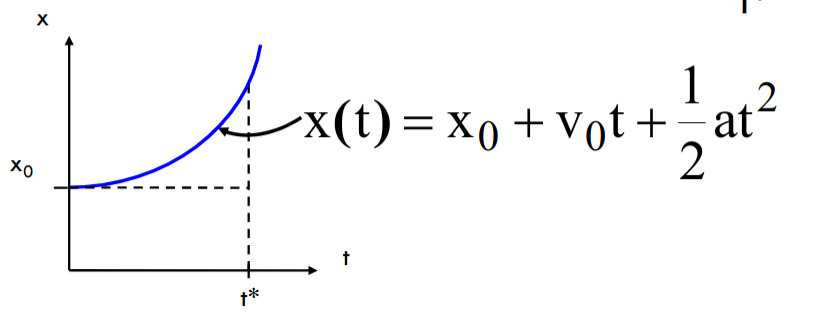
\includegraphics[width=0.8\textwidth]{mrua_leggeoraria}
	\end{figure}
	\subsection{Accelerazione di gravita'}
	Se lanciando un oggetto verso l'alto o verso il basso si riuscisse in qualche modo a eliminare l'effetto dell'aria sul moto dell'oggetto, si troverebbe che la sua accelerazione verso il basso ha un valore costante ben definito. Questa accelerazione e' chiamata \textbf{accelerazione in caduta libera} o \textbf{accelerazione di gravita'} e il suo modulo e' indicato con $g$ che e' uguale per qualsiasi oggetto. Il valore di $g$ varia leggermente con la latitudine e anche con la quota. Al livello del mare, alle latitudini medie:
	\[
	g = 9,8 \ m/s^2
	\]
	L'accelerazione di gravita' in prossimita' della superficie terreste vale:
	\[
	a = -g = -9,8 \ m/s^2
	\]
	\begin{example}{\nmu Caduta libera di un grave}{mrua_caduta_grave}
	(Vedere dalle slide)
	\end{example}
	
	
	\chapter{Cinematica in due e tre dimensioni}
	\section{Posizione e spostamento nel moto piano}
	Un modo comune per localizzare una particella e' tramite il \textbf{vettore posizione r}, un vettore che ha origine in un punto di riferimento e arriva al punto in cui la particella si trova. Nella notazione dei versori, \textbf{r} puo' essere scritto come:
	\[
	\textbf{r} = x\textbf{i} + y\textbf{j} + z\textbf{k}
	\]
	dove $x\textbf{i}$, $y\textbf{j}$ e $z\textbf{k}$ sono le componenti vettoriali di \textbf{r} e i coefficienti $x, y, z$ sono le sue compoenenti scalari. \\
	Le componenti scalari danno la posizione della particella lungo gli assi coordinati e relativamente all'origine.\\
	Quando una particella si muove, il suo vettore posizione cambia in modo da estendersi sempre dal punto di riferimento verso la particella. Se il vettore posizione, ad esempio, cambia da $\mathbf{r_1}$ a $\mathbf{r_2}$ in un certo intervallo di tempo, allora il vettore \textbf{spostamento} $\Delta\textbf{r}$ della particella durante quell'intervallo di tempo e':
	\[
	\Delta\textbf{r} = \textbf{r}_2 - \textbf{r}_1
	\]
	usando la notazione dei versori otteniamo:
	\[
	\Delta \textbf{r} = (x_2\textbf{i}+y_2\textbf{j}+z_2\textbf{k}) - (x_1\textbf{i}+y_1\textbf{j}+z_1\textbf{k})
	\]
	e possiamo riscrivere il vettore spostamento come:
	\[
	\Delta \textbf{r} = \Delta x \textbf{i} + \Delta y \textbf{j} + \Delta z\textbf{k}
	\]
	La situazione e' quella mostrata in figura:
	\section{Velocita' media e istantanea di un moto piano}
	Se una particella si muove da un punto a un altro, potremmo aver bisogno di sapere quanto velocemente si muova e come per il moto uniforme ci sono due tipologie di velocita':
	\begin{enumerate}
		\item \textbf{velocita' media};
		\item \textbf{velocita' istantanea}.
	\end{enumerate}
	\paragraph{Velocita' media}\quad \\ Se una particella compie uno spostamento $\Delta \textbf{r}$ in un intervallo di tempo $\Delta t$, la sua \textit{velocita' vettoriale media} $\mathbf{v_m}$ e':
	\[
	\mathbf{v_m} = \frac{\Delta \textbf{r}}{\Delta t}
	\]
	Questo ci dice che la direzione di $\mathbf{v_m}$ deve essere la stessa del vettore spostamento. Possiamo riscrivere la velocita' media in termini delle componenti vettoriali di \textbf{r}:
	\[
	\mathbf{v_m} = \frac{\Delta x \textbf{i} + \Delta y \textbf{j} + \Delta z\textbf{k}}{\Delta t} = \frac{\Delta x}{\Delta t}\textbf{i} + \frac{\Delta y}{\Delta t}\textbf{j}+ \frac{\Delta z}{\Delta t}\textbf{k}
	\]
	\paragraph{Velocita' istantanea}\quad \\ Quando parliamo di \textbf{velocita'} di una particella, intendiamo la \textbf{velocita' istantanea v} della particella in un dato istante. Questa \textbf{v} e' il valore al quale $\mathbf{v_m}$ si avvicina nel limite in cui restringiamo l'intervallo di tempo $\Delta t$ attorno all'istante dato. Possiamo scrivere \textbf{v} come:
	\[
	\textbf{v} = \lim_{\Delta t \to 0}\frac{\Delta \textbf{r}}{\Delta t} = \frac{d\textbf{r}}{dt} 
	\]
	Utilizzando la notazione con i versori:
	\[
	\textbf{v} = \frac{dx}{dt}\textbf{i} + \frac{dy}{dt}\textbf{j}+\frac{dz}{dt}\textbf{k} = v_x\textbf{i}+v_y\textbf{j}+v_z\textbf{k}
	\]
	ove $v_x, v_y$ e $v_z$ sono le componenti scalari di \textbf{v} e possiamo trovarle derivando le componenti scalari di \textbf{r}
	\section{Accelerazione media e accelerazione istantanea}
	\paragraph{Accelerazione media} \quad \\
	Quando la velocita' di una particella cambia da $\mathbf{v_1}$ a $\mathbf{v}_2$ in un intervallo di tempo $\Delta t$, la sua \textbf{accelerazione media} $\mathbf{a_m}$ nell'intervallo di tempo $\Delta t$ e':
	\[
	\mathbf{a_m} = \frac{\mathbf{v_2} - \mathbf{v_1}}{\Delta t} = \frac{\Delta \textbf{v}}{\Delta t}
	\]
	\paragraph{Accelerazione istantanea} \quad \\
	Se riduciamo l'intervallo di tempo $\Delta t$ a zero attorno a un dato istante, $\mathbf{a_m}$ tende all'\textbf{accelerazione istantanea} o \textbf{accelerazione a} all'istante considerato, cioe':
	\[
	\textbf{a} = \lim_{\Delta t\to 0}\frac{\Delta \textbf{v}}{\Delta t}=\frac{d\textbf{v}}{dt} = \frac{dv_x}{dt}\textbf{i} + \frac{dv_y}{dt}\textbf{j} + \frac{dv_z}{dt}\textbf{k} = a_x\textbf{i} + a_y\textbf{j} + a_z\textbf{k}
	\] 
	Quindi per trovare le componenti scalari di \textbf{a}, $a_x, a_y, a_z$, deriviamo le componenti scalari di \textbf{v}.
	\begin{note}{\nmu Direzione e verso del vettore accelerazione}{dir_ver_acc}
		E' bene notare che il vettore accelerazione \textbf{a}, non ha, in generale, la stessa direzione e lo stesso verso dei vettori velocita' e spostamento.
	\end{note}
	\section{Moto di un proiettile}
	Consideriamo ora un caso particolare: una particella si muove nel piano verticale con una qualche velocita' iniziale $\mathbf{v_0}$ ma la sua accelerazione e' sempre l'accelerazione \textbf{g} del moto in caduta libera. Tale particella e' chiamata \textbf{proiettile} e il suo moto e' chiamato \textbf{moto del proiettile}.  \\
	Il proiettile e' lanciato con una velocita' iniziale $\mathbf{v_0}$ che si puo' esprimere come:
	\[
	\mathbf{v_0}=v_{0_x}\textbf{i} + v_{0_y}\textbf{j}
	\]
	La situazione e' quella in figura:
	\begin{figure}[H]
		\centering
		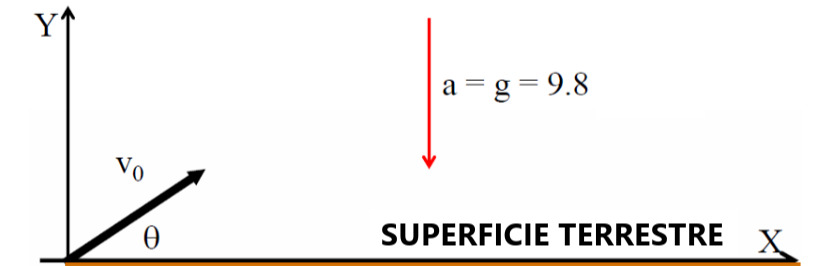
\includegraphics[width=0.45\textwidth]{moto_del_proiettile}
	\end{figure}
	Conoscendo l'angolo $\theta$ tra $\mathbf{v_0}$ e il verso positivo dell'asse $x$, possiamo ricavare le componenti $v_{0_x}$ e $v_{0_y}$:
	\[
	v_{0_x} = v_0\cos \theta \quad v_{0_y}=v_0\sin \theta
	\]
	Durante il moto, il vettore posizione \textbf{r} e il vettore velocita' \textbf{v} del proiettile cambiano continuamente, ma il suo vettore accelerazione ha sempre modulo costante ed e' sempre diretto verso il basso. Il moto del proiettile sembra complicato ma ha una caratteristica che semplifica le cose:
	\begin{note}{}{}
		Nel moto di un proiettile il moto orizzontale e il moto verticale sono indipendenti l'uno dall'altro; nessuno dei due moti influenza l'altro.
	\end{note}
	Questa proprieta' ci permette di suddividere il problema in due problemi separati e piu' semplici in quanto sono in una sola dimensione, uno per il moto orizzontale con accelerazione nulla e l'altro per il moto verticale con accelerazione costante verso il basso. \\
	Siamo ora in grado di analizzare il moto di un proiettile, orizzontalmente e verticalmente.
	\paragraph{Moto orizzontale} \quad \\
	Dal momento che non c'e' accelerazione nella direzione orizzontale, la componente orizzontale $v_x$ delle velocita' del proiettile rimane invariata rispetto al valore iniziale $v_{0_x}$ durante tutto il moto. Ad ogni istante $t$, lo spostamento orizzontale $x - x_0$ del proiettile e' dato dall'equazione del moto rettilineo uniforme con $a = 0$, che scriviamo come:
	\[
	x - x_0 = v_{0_x}t
	\]
	poiche' $v_{0_x} = v_0\cos \theta$ si ha:
	\[
	x - x_0 = (v_0\cos \theta)t
	\]
	\paragraph{Moto verticale} \quad \\
	Il moto verticale e' l'equazione del moto uniformemente accelerato con accelerazione costante. Quindi sostituendo $a$ con $-g$ e passando alla notazione con $y$, l'equazione diventa:
	\[
	y-y_0 = v_{0_y}t-\frac{1}{2}gt^2 = (v_0\sin \theta)t-\frac{1}{2}gt^2
	\]
	Le equazioni della velocita' diventano:
	\[
	v_y = v_0\sin\theta - gt \quad v_x = v_0\cos\theta
	\]
	\paragraph{Equazione della traiettoria} \quad \\
	Possiamo trovare l'equazione della \textbf{traiettoria} del proiettile supponendo che il proiettile parta dall'orgine del sistema di riferimento $x_0 = y_0 = 0$ e possiamo ricavare l'equazione partendo dalle leggi orarie ed eliminando la dipendenza dal tempo:
	\[
	\begin{cases}
		t = \frac{x}{v_{0_x}} \\
		y = v_{0_y} \cdot \frac{x}{v_{0_x}}-\frac{1}{2}g\frac{x^2}{v_{0_x}^2} 
	\end{cases} \Rightarrow y = -\frac{1}{2}g\frac{x^2}{v_{0_x}^2} + \frac{v_{0_y}}{v_{0_x}}x
	\]
	ove $y$ e' l'equazione di una parabola con concavita' rivolta verso il basso.
	\begin{figure}[H]
		\centering
		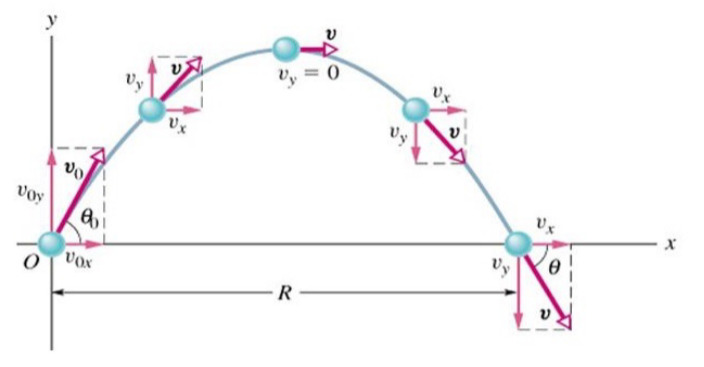
\includegraphics[width=0.65\textwidth]{traiettoria_proiettile}
	\end{figure}
	\begin{itemize}
		\item $v_x$ resta costante a $v_{0_x}$, $v_y$ decresce costantemente nel tempo;
		\item Nel punto piu' alto della traiettoria $v_y = 0$
		\item Nel punto di caduta si ha $v_y = -{v_{0_y}}$
	\end{itemize}
	\paragraph{Altezza massima} \quad \\
	\begin{itemize}
		\item Quanto vale l'altezza massima raggiunta dal corpo? \\
		Quando il corpo raggiunge il punto di massima altezza la sua velocita' lungo l'asse verticale si annulla:
		\[
		v_y = v_{0_y} - gt = 0
		\]
		\item Da quella relazione possiamo ricavare il tempo impiegato a raggiungere l'altezza massima $t=t_{max}$:
		\[
		t_{max} = v_{0_y}/g
		\]
		\item Infine, dall'equazione del moto possiamo determinare l'\textbf{altezza massima}:
		\[
		y=v_{0_y}t-\frac{1}{2}gt^2 = v_{0_y}\frac{v_{0_y}{g}}-\frac{1}{2}g\frac{v_{0_y}^2}{g^2} = \frac{1}{2}\frac{v_{0_y}^2}{g}
		\]
	\end{itemize}
	\paragraph{Gittata} \quad \\
	La \textit{gittata R} di un proiettile e' la distanza \textit{orizzontale} che il proiettile ha perecorso quando ritorna alla quota di partenza. Dalla definizione, per trovare la formula della gittata basta calcolare, dall'equazione della parabola, il valore di $x$ per $y=0$:
	\[
	\begin{cases}
		y=-\frac{1}{2}\frac{g}{v_{0_x}^2}x^2+\frac{v_{0_y}}{v_{0_x}}x \\
		y=0
	\end{cases} \Rightarrow \begin{cases}
		y=-\frac{1}{2}\frac{g}{(v_{0}\cos\theta)^2}x^2+\frac{v_{0}\sin\theta}{v_{0}\cos\theta}x \\
		y=0
	\end{cases}
	\] 
	Quindi otteniamo:
	\[
	0 = -\frac{g}{2v_0^2\cos^2\theta}x^2 + \tan\theta \cdot x
	\]
	Un equazione di secondo grado del tipo $ax^2+bx = 0$ le cui soluzioni sono $x_1 = 0$ e $x_2 = -b/a$, il nostro $x_2$ e':
	\[
	x_2 = -\frac{\sin\theta}{\cos\theta} \cdot \frac{2v_0^2\cos^2\theta}{g} = \frac{v_0^2}{g}2\sin\theta\cos\theta = \frac{v_0^2}{g}\sin(2\theta)
	\]
	\section{Moto circolare uniforme}
	Una particella compie un \textit{moto circolare uniforme} se si muove su una circonferenza o su un arco di circonferenza con una velocita' di modulo costante. Sebbene il modulo della velocita' non cambia, la particella \textit{accelera} perche' cambia la direzione della sua velocita'. \\
	\begin{figure}[H]
		\centering
		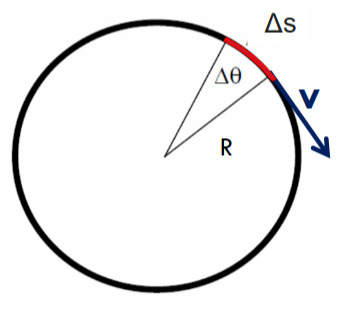
\includegraphics[width=0.5\textwidth]{moto_circolare_uniforme}
	\end{figure}
	Entrambi i vettori, il vettore velocita' e accelerazione, hanno modulo costante ma le loro direzione e versi cambiano continuamente. La velocita' e' sempre diretta lungo la tangente alla circonferenza nel verso del moto. L'accelerazione e' sempre diretta \textit{lungo il raggio e verso il centro}. Per questo motivo l'accelerazione associata al moto circolare unirforme e' detta \textbf{accelerazione centripeta}. Il modulo di accelerazione di $\vec{a}$ e' dato da:
	\[
	a = \frac{v^2}{r}
	\]
	dove $r$ e' il raggio della circonferenza e $v$ e' il modulo della velocita'. Inoltre, durante questa accelerazione con modulo della velocita' costante, la particella percorre la circonferenza nel tempo:
	\[
	T = \frac{2\pi r}{v}
	\]
	$T$ e' chiamato \textit{periodo di rivoluzione} o semplicemente \textit{periodo del moto}. \\
	Introduciamo le coordinate angolari:
	\begin{itemize}
		\item la posizione angolare $\theta$ si misura in rad:
		\[
		\theta = \frac{s}{r}
		\]
		\item la velocita' angolare $\omega$ si misura in rad/s:
		\[
		\omega_m = \frac{\Delta \theta}{\Delta t} = \frac{2\pi}{T}
		\]
	\end{itemize}
	La relazione tra velocita' angolare e lineare e':
	\[
	v = \frac{\Delta s}{\Delta t} = \frac{r\Delta \theta}{\Delta t} = \omega r
	\]
	Possiamo scrivere l'equazione oraria per un moto circolare uniforme usando le coordinate angolari:
	\[
	\theta = \theta_0 + \omega(t - t_)
	\]
	\[
	\omega = const
	\]
	\[
	a = \frac{v^2}{r} = \frac{(\omega r)^2}{r} = \omega^2 r
	\]
	Usando un sistema di riferimento dedicato, come mostrato nella figura:
	\begin{figure}[H]
		\centering
		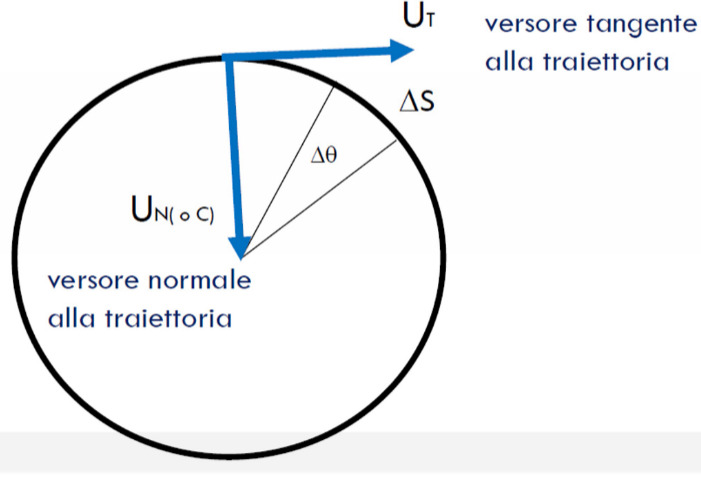
\includegraphics[width=0.5\textwidth]{circolare_sistema_dedicato}
	\end{figure}
	possiamo riscrivere le formule scritte precedentemente in termini vettoriali:
	\[
	a = \frac{v^2}{r}\mathbf{u_n} = \omega^2 r \mathbf{u_n}
	\]
	quella centripeta, $\mathbf{u_n}$, e' l'unica componente dell'accelerazione in un moto circolare uniforme, ed e' legata alla variazione della direzione della velocita' istantanea, quindi, non c'e' nessuna componente in direzione tangenziale $\mathbf{u_T}$. \\
	\paragraph{Moto circolare non uniforme} \quad \\
	Nel caso di moto circolare non uniforme anche il modulo della velocita' varia. Esiste dunque un'altra componente dell'accelerazione, chiamata \textit{accelerazione tangenziale}:
	\[
	\mathbf{a_T} = \frac{d|v|}{dt}\mathbf{u_T}
	\]
	legata alla variazione del solo modulo della velocita'. \\
	Si puo' quindi scrivere complessivamente, l'accelerazione vettoriale come la somma delle due componenti:
	\[
	\vec{a} = \frac{d|v|}{dt}\vec{u_T} + \frac{v^2}{r}\vec{u_N}
	\]
	ove l'accelerazione tangenziale descrive la variazione del modulo di $\vec{v}$ e l'accelerazione centripeta descrive la variazione della direzione di $\vec{v}$.\\
	Possiamo infine definire l'accelerazione angolare:
	\[
	\alpha = \frac{d\omega}{dt}
	\]
	e si dimostra che l'accelerazione angolare e' legata alla sola accelerazione tangenziale:
	\[
	\alpha_T = \alpha r
	\]
	In definitiva l'accelerazione vettoriale puo' essere scritta nel seguente modo:
	\[
	\vec{a} = \frac{d|v|}{dt}\vec{u_T} + \frac{v^2}{r}\vec{u_N} = \alpha r \vec{u_T} + \frac{v^2}{r}\vec{u_N}
	\]
	\section{Moto circolare uniformente accelerato} 
	Un caso particolare di moto circolare non uniforme e' quello uniformemente accelerato. Usando le coordinate angolari, le equazioni sono analoghe al caso rettilineo:
	\[
	\alpha = const
	\]
	\[
	\omega = \omega_0 + \alpha(t -t_0)
	\]
	\[
	\theta = \theta_0 + \omega_0(t - t_0) + \frac{1}{2}\alpha(t - t_0)^2
	\]
	\subsection{Moto armonico semplice}
	\begin{figure}[H]
		\centering
		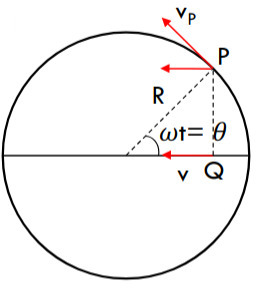
\includegraphics[width=0.5\textwidth]{moto_armonico_semplice}
	\end{figure}
	Consideriamo un punto $P$ che si muove di moto circolare unforme e proiettiamo lungo gli assi cartesiani $X-Y$. \\
	Si definisce \textit{moto armonico} il moto del punto di proiezione $Q$, cioe' la proiezione del punto $P$ sull'asse $X$. \\
	La proiezione del punto $P$ sull'asse $X$ e' dato da:
	\[
	x = R \cos\theta
	\]
	Ricordando che nel moto circolare uniforme l'equazione oraria e' $\theta=\theta_0 + \omega t$, l'equazione oraria di un moto armonico e':
	\[
	x(t) = R \cos (\omega t + \theta_0)
	\]
	Il moto armonico e' un moto rettilineo ed e' descritto dalle funzioni seno e coseno e in generale l'equazione di un moto armonico e':
	\[
	x(t) = A \sin (\omega t + \phi_0)
	\]
	ove $A$ e' detta \textbf{ampiezza}, $\omega$ e' detta \textbf{pulsazione} e $\phi_0$ e' la \textbf{fase iniziale}. \\
	Il moto armonico semplice e' un moto periodico, il cui periodo coincide con quello del moto circolare:
	\[
	T = \frac{2\pi}{\omega}
	\]
	Si definisce \textbf{frequenza} e si misura in Hertz, [Hz] = [1/s]:
	\[
	v = \frac{1}{T} = \frac{\omega}{2\pi}
	\]
	Infine, si puo' dimostrare la seguente relazione, che e' caratteristica di questo tipo di moto:
	\[
	a(t) = -\omega^2x(t)
	\]
	\chapter{Forza e moto}
	\section{Introduzione alla dinamica}
	La \textbf{dinamica} e' il ramo della meccanica che si occupa dello studio delle \textit{cause} del moto dei corpi o, in altri termini, delle circostanze che lo determinano e lo modificano.\\
	La dinamica si divide in:
	\begin{itemize}
		\item \textit{Dinamica del punto materiale}:
		\begin{enumerate}
			\item \textbf{I parte:} Principi della dinamica;
			\item \textbf{II parte}: Classificazione delle forze.
		\end{enumerate}
		\item \textit{Dinamica dei sistemi di punti materiali}. \\
		Estensione della dinamica del punto materiale a sistemi estesi come sistemi di punti, corpi rigidi, ecc. 
	\end{itemize}
	Ricordiamo che un punto materiale e' corpo privo di dimensioni o che presenta dimensioni trascurabili rispetto a quelle dello spazio in cui puo' muoversi o degli altri corpi con cui puo' interagire. In generale un punto materiale e' solamento caratterizzato dalle \textit{coordinate spaziali}, da \textit{velocita'} ed \textit{accelerazione} e dalla sua \textit{massa}. L'utilita' del concetto di punto materiale sta nel poter associare al corpo un punto geometrico nello spazio, ma e' solo un modello. \\
	La dinamica spiega il perche' i corpi cambiano il loro stato di moto e che cosa imprime loro un'accelerazione. Per fare cio' vengono introdotte due nuove grandezze fisiche:
	\begin{enumerate}
		\item \textbf{Forza};
		\item \textbf{Massa}.
	\end{enumerate}
	Esiste un legame \textit{forza-accelerazione} e Galielo afferma che la forza determina una variazione del moto ma non il moto stesso, in quanto un corpo puo' restare in moto anche senza forze applicate e si puo' usare una forza anche per arrestare un moto.
	\section{Forza}
	Una \textit{forza}, generalmente parlando, e' una spinta o una trazione applicata all'oggetto che causa l'accelerazione di quest'ultimo. Si dice che la forza agisce sull'oggetto per modificarne la velocita'. \\
	Quindi, la forza e' una qualsiasi causa esterne che perturba lo stato di quiete o di moto rettilineo uniforme. Questa e' una definizione qualitativa perche' non e' ancora stato introdotto la procedura per la misura della grandezza fisica della forza.
	\subsection{Prima legge della dinamica}
	La prima legge della dinamica afferma che:
	\begin{center}
		\textit{Ogni corpo persiste nello stato di quiete o di moto rettilineo uniforme finche' delle forze non intervengono a mutare tale stato}
	\end{center}
	E' bene notare che assenza di forze non significa che non c'e' moto, ma significa che la velocita' non varia. \\
	La tendenza di un corpo a mantenere il suo stato di quiete o di moto rettilineo uniforme e' chiam\textbf{inerzia} e per questo il primo principio della dinamica e' anche chiamato \textbf{principio di inerzia}. \\
	Da questo, possiamo completare la formulazione della prima legge della dinamica:
	\begin{center}
		\textit{In un sistema di riferimento inerziale, ogni corpo persiste nello stato di quiete o di moto rettilineo uniforme finche' delle forze non intervengono a mutare tale stato}
	\end{center}
	Quindi, la prima legge della dinamica e' valida solo in una particolare classe di sistemi di riferimento, detti \textit{sistemi di riferimento inerziali}. \\
	Per esempio, possiamo supporre che il terreno sia un sistema inerziale purche' si possano trascurare gli effetti del moto astronomico della Terra. Questa ipotesi funziona bene se, per esempio, facciamo scivolare un disco da hockey lungo un \textit{breve} tratto di ghiaccio privo di attrito e noteremmo che il moto del disco obbedisce alla prima legge della dinamica. Ma, supponendo che il disco venga fatto scivolare per un lungo tratto che parte dal polo nord, se guardiamo il disco da un sistema di riferimento in quiete nello spazio, vediamo che si muove lungo una semplice linea retta. Se invece vediamo il disco da un punto a terra in modo tale che noi ruotiamo con la Terra, la sua traiettoria non e' una semplice linea retta in quanto la velocita' verso est del suoto sotto al disco e' maggiore quanto piu' il disco scivola verso sud e dal nostro punto di riferimento appare deviato verso ovest. Ma, questa deviazione non e' provocata da una forza, ma dal fatto che vediamo il disco da un sistema di riferimento che ruota, quindi il terreno e' un \textit{sistema di riferimento non inerziale}.
	\subsection{Seconda legge della dinamica} Supponendo di imprimere una forza ad un corpo, la forza imprime al corpo un'accelerazione ed e' possibile misurare una forza dall'accelerazione che produce sul corpo.
	Il secondo principio della dinamica di che:
	\begin{center}
		\textit{Una forza }\textbf{F} \textit{applicata ad un corpo libero di muoversi imprime un'accelerazione} \textbf{a} \textit{nella stessa direzione e nello stesso verso della forza applicata ed inoltre}:
		\[
		\mathbf{F} = m\mathbf{a}
		\]
	\end{center}
	La costante di proporzionalita' tra \textbf{F} ed \textbf{a} e' la \textit{massa}. \textbf{F} ed \textbf{a} sono grandezze vettoriali e $m$ e' una grandezza scalare.
\end{document}
